\title{Improving migration resolution by approximating the least-squares Hessian using non-stationary amplitude and frequency matching}

\usetikzlibrary{arrows,automata}
\author{Sarah Greer*, Zhiguang Xue, and Sergey Fomel, The University of Texas at Austin}
\label{ch:chapter-mighes}

\relax\footnotetext{Parts of this chapter were first published in \cite{mighess}. This work was done under the supervision of Dr. Sergey Fomel, and Dr. Zhiguang Xue assisted in the migration of the Sigsbee synthetic data set.}

\newcommand*{\tran}{^{\mkern-1.5mu\mathsf{T}}}
\maketitle
\inputdir{sigsbee}
\begin{abstract}
    We propose using two non-stationary operators to represent the amplitude and frequency variations in the least-squares Hessian to account for the principal differences between conventional and least-squares migrated images.
    The calculation and application of these operators are computationally inexpensive when compared to one iteration of least-squares migration, and it increases the resolution and amplitude fidelity of the migrated image.
    Successful results are achieved on an application of reverse-time migration to the Sigsbee synthetic data set.
\end{abstract}

\section{Introduction}
    Least-squares migration can produce an accurate migrated seismic image.
    However, the process may be computationally expensive as it is typically performed in an iterative manner, where each iteration involves forward modeling and migration. 
    Although conventional seismic migration is less computationally expensive than least-squares migration, it generally contains migration artifacts affecting amplitude fidelity and resolution \cite[]{lsamp,pwlsrtm}.
    This can be attributed to the fact that, while least-squares migration inverts for subsurface reflectivity by finding the least-squares model solution, standard migration amounts to applying a single adjoint operation \cite[]{pvi}. 

    Various methods have attempted to correct these differences by finding and applying an approximation to the inverse Hessian operator, $\mathbf{H}^{-1} = \left (\mathbf{L}\tran\mathbf{L} \right )^{-1}$, to a conventional migrated image.
    Here, $\mathbf{L}$ is a standard forward-modeling operator, and $\mathbf{L}\tran$ is its adjoint---the migration operator.
    These methods usually take the form of two approaches---for preconditioning before least-squares migration and as a single operation to improve accuracy of a conventionally migrated image.
    Previously, this has been done by migration deconvolution \cite[]{poststack,prestack}, approximating the diagonal of $\mathbf{H}^{-1}$ to account for amplitude effects \cite[]{amp,diagamp}, and by finding and applying a bank of non-stationary matching filters \cite[]{imop,rtmmf} or deblurring filters \cite[]{debfilt} to a conventionally migrated image.
    This traditionally is done using a sliding window approach, where windowed regions and partial overlap regions are specified, and different matching filters are specified in each region \cite[]{seiinv}.

    In this thesis, we take a different approach. 
    We note that the two primary differences between least squares migrated images and conventional migrated images are amplitude and frequency variations \cite[]{Hou2015, Hou2016}. 
    Here, we treat this as a data matching problem between two conventionally migrated images, and find separate operations to account for both amplitude and frequency variations.

    This approach enables us to rely on local seismic attributes to measure and apply amplitude and frequency balancing operations instead of using a sliding window approach \cite[]{attr}.
This allows for the smooth estimation and application of these matching operations instead of applying them in discrete windows.
    Because the operations for balancing amplitude and frequency content are calculated and applied separately from each another, the effect of each operation can be adjusted independently, which is another advantage of the proposed method.
    To test the proposed approach, we apply this method to an example of reverse-time migration on the Sigsbee synthetic data set \cite[]{sigsbee}. 

\section{Theory}
    The goal of least-squares migration is to find the image, $\hat{\mathbf{r}}$, that minimizes
    \begin{equation}
        p(\hat{\mathbf{r}}) = \frac{1}{2}\left \Vert \mathbf{\mathbf{d} - L\hat{r}} \right \Vert _2^2\;,
        %p(\hat{\mathbf{r}}) = \frac{1}{2}\left \lVert \mathbf{\mathbf{d} - L\hat{r}} \right \rVert _2^2\;,
    \end{equation}
    where $\mathbf{L}$ is the forward modeling operator, representing seismic wave propagation through the subsurface, and $\mathbf{d}$ is the acquired seismic data.
    This can be solved by the least-squares formulation to find $\hat{\mathbf{r}}$:
    \begin{equation}
        \hat{\mathbf{r}} = \left ( \mathbf{L}\tran\mathbf{L}\right )^{-1}\mathbf{L}\tran\mathbf{d}\;,
        \label{eq:ls}
    \end{equation}
    where the migration operator, $\mathbf{L}\tran$, is adjoint to the forward modeling operator and is typically sparse, and $\left ( \mathbf{L}\tran \mathbf{L} \right )^{-1}$ is the inverse Hessian operator.
    Equation (\ref{eq:ls}) is usually solved iteratively, typically requiring multiple iterations of forward modeling and remigrating the seismic image \cite[]{wem,xue16}. 
Conventional migration is less computationally expensive:
\begin{equation}
    \mathbf{m}_0 = \mathbf{L}\tran\mathbf{d}.
    \label{eq:mod}
\end{equation}
    However, conventionally migrated images generally exhibit less correct amplitude and frequency content than least-squares migrated images \cite[]{dutta14}. 
    By combining equations (\ref{eq:ls}) and (\ref{eq:mod}), it is evident that
\begin{equation}
    \hat{\mathbf{r}} = \left ( \mathbf{L}\tran\mathbf{L}\right )^{-1}\mathbf{m}_{0} \;,
\end{equation}
    so $\mathbf{m}_0$ is a distorted version of $\hat{\mathbf{r}}$, and $\hat{\mathbf{r}}$ can be recovered from $\mathbf{m}_0$ by finding a good approximation of $\left ( \mathbf{L}\tran\mathbf{L}\right) ^{-1}$.

\section{Method}
    In order to approximate $\left ( \mathbf{L}\tran\mathbf{L}\right) ^{-1}$, we follow the modeling and remigration process of \cite{imop}. 
    We begin by forward modeling the migrated image, $\mathbf{m}_0$:
    \begin{equation}
        \mathbf{d}_1 = \mathbf{L}\mathbf{m}_0 \;.
    \end{equation}
    We then remigrate $\mathbf{d}_1$:
    \begin{equation}
        \mathbf{m}_1 = \mathbf{L}\tran\mathbf{d}_1 = \left ( \mathbf{L}\tran\mathbf{L}\right ) \mathbf{m}_0 \; ,
    \end{equation}
    and then find the operator, $\left ( \mathbf{L} \tran \mathbf{L} \right )^{-1}$, that satisfies
    \begin{equation}
        \mathbf{m}_0 = \left ( \mathbf{L}\tran\mathbf{L} \right ) ^{-1} \mathbf{m}_1 \;.
    \end{equation}
    Therefore, the inverse Hessian operator, $\mathbf{H}^{-1} = \left ( \mathbf{L} \tran \mathbf{L} \right )^{-1}$, that must be applied to $\mathbf{m}_0$ to obtain $\hat{\mathbf{r}}$ can be calculated by first finding the transformation, $\mathbf{H}$, that maps $\mathbf{m}_0$ to $\mathbf{m}_1$, and then inverting it.
    This can be interpreted as a data matching problem between $\mathbf{m}_1$ and $\mathbf{m}_0$.

\begin{center}
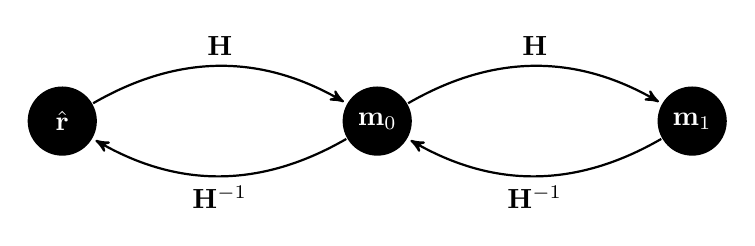
\begin{tikzpicture}[auto,node distance=4cm,thick, ->, >=stealth',shorten >=1pt]
  \tikzstyle{every state}=[fill=black,draw=none,text=white]

        \node[state]         (A)              {$\mathbf{m}_0$};
        \node[state]         (B) [right of=A] {$\mathbf{m}_1$};
        \node[state]         (C) [left of=A]  {$\hat{\mathbf{r}}$};

        \path (A) edge [bend left] node {$\mathbf{H}$} (B)
            edge [bend left] node {$\mathbf{H}^{-1}$} (C)
        (B) edge [bend left] node {$\mathbf{H}^{-1}$} (A)
        (C) edge [bend left] node {$\mathbf{H}$} (A);

\end{tikzpicture}
\end{center}


    \multiplot{2}{mod,vel-migration}{width=0.85\columnwidth}{The Sigsbee model reflectivity (a), and migration velocity model (b).}
    \multiplot{2}{image0,image1}{width=0.85\columnwidth}{The first migrated image, $\mathbf{m}_0$ (a), and the second migrated image, $\mathbf{m}_1$ (b).}
%\multiplot{4}{mod,vel-migration,image0,image1}{width=0.98\columnwidth}{The Sigsbee model reflectivity (a), migration velocity model (b), the first migrated image, $\mathbf{m}_0$ (c), and the second migrated image, $\mathbf{m}_1$ (d).}
    Because the primary differences between conventionally migrated images and least-squares migrated images amount to amplitude and frequency variations, we use two separate non-stationary operators to represent the forward Hessian---one to account for amplitude variations, and the other to account for frequency variations. 
    Therefore, our approximation of $\mathbf{H}$ can be calculated from some application of a non-stationary amplitude balancing operator, $\mathbf{A}$, and a non-stationary frequency balancing operator, $\mathbf{S}$.
    We first calculate the forward Hessian because the forward frequency balancing operation, $\mathbf{S}$, is well defined and simple to calculate. 
    We then invert our approximation to the Hessian and apply it to $\mathbf{m}_0$ to correct the amplitude and frequency content of the migrated image.

\subsection{Amplitude operator}
    First, we choose to find an amplitude balancing operation that, when applied to $\mathbf{m}_0$, balances the amplitudes of $\mathbf{m}_0$ with respect to $\mathbf{m}_1$. 
    This operation can be equated to a trace-by-trace multiplication of a diagonal matrix to each trace, where the matrix changes for every trace.
    We estimate it by first calculating the amplitude envelope of the traces in $\mathbf{m}_0$ and $\mathbf{m}_1$, and then smoothly dividing them.
    The corresponding diagonal weighting operator, $\mathbf{A}$, can be applied such that $\mathbf{m}_1 \approx \mathbf{A}\mathbf{m}_0$ to balance the amplitudes of each trace.
    Because this is a linear operation that only has diagonal elements, finding the inverse operator, $\mathbf{A}^{-1}$ is trivial. 

\subsection{Frequency operator}
    In addition to amplitude corrections, we also attempt to account for the decrease in resolution of a conventional migrated image compared to its corresponding least-squares migrated image. 
    This loss in resolution can be equated to the fact that $\mathbf{L}\tran\mathbf{L}$ acts as a blurring operator, where the conventional migrated image is a blurred version of the ideal least-squares migrated image \cite[]{poststack}. 
    We choose to approximate this blurring using non-stationary triangle smoothing.

    We begin by first calculating the local frequency of the two initial images \cite[]{attr}. 
    Local frequency is a temporally and spatially varying frequency attribute that smoothly varies across the image without windows.
    Our goal is to find a transformation that we can apply to $\mathbf{m}_0$ that matches the local frequency content with $\mathbf{m}_1$. 
    To do this, we propose using non-stationary triangle smoothing. 
    This approach involves finding and applying a non-stationary smoothing operator, which is the number of samples, in both dimensions, that $\mathbf{m}_0$ will be averaged over in a triangle weight, to balance the local frequency content with $\mathbf{m}_1$. 
    
    We find the smoothing radius iteratively using the method of \cite{locfreq} from Chapter \ref{ch:chapter-locfreq}, with a modification that allows the smoothing radius to be calculated in both spatial directions. 
Essentially, this is found by choosing an initial guess of a smoothing radius, $\mathbf{R}^{(0)}$, and updating it iteratively such that 
    \begin{equation}
        \label{eq:it}
        \mathbf{R}^{(i+1)} = \mathbf{R}^{(i)}+ \alpha \left [ \mathbf{F}[\mathbf{S}_{\mathbf{R}^{(i)}} \mathbf{m}_0] - \mathbf{F}[\mathbf{m}_1] \right ]\;,
    \end{equation}
    where $\mathbf{F}$ is the local frequency operator, $\mathbf{S}_{\mathbf{R}^{(i)}}$ is the smoothing operator of radius $\mathbf{R}$ at the $i$th iteration, and $\alpha$ is a scalar constant that represents the step length.
    After a small number of iterations, the smoothing operator is found that, once applied to $\mathbf{m}_0$, balances local frequency content with $\mathbf{m}_1$.

    For this particular application using depth migration, this operator should technically be specified to balance {\em wavenumber} instead of {\em frequency}.
    However, it is kept as frequency to keep consistent terminology with the algorithm developed in Chapter \ref{ch:chapter-locfreq}.

    \multiplot{2}{a0,rect10b}{width=0.85\columnwidth}{The forward amplitude balancing weight, $\mathbf{A}$ (a) and the smoothing radius (b), which represents the number of samples in both dimensions that $\mathbf{m}_0$ must be smoothed over in a triangle weight to balance the local frequency content with $\mathbf{m}_1$. This represents the forward smoothing operation, $\mathbf{S}$.}

\subsection{Calculating the inverse Hessian}
    Now that we have found the forward operators that separately balance amplitude and frequency content from $\mathbf{m}_0$ to $\mathbf{m_1}$, where $\mathbf{m}_1 \approx \mathbf{H} \mathbf{m}_0$, we want to find what combination of $\mathbf{A}$ and $\mathbf{S}$ best approximates $\mathbf{H}$.
    Since $\mathbf{H} = \mathbf{L}\tran\mathbf{L}$ is symmetric, we want our approximation of $\mathbf{H}$ to be as close to symmetric as possible.
    Therefore, we define $\mathbf{H}$ as
    \begin{equation}
        \mathbf{H} \approx \mathbf{A}^{\sfrac{1}{2}}\mathbf{S}\mathbf{A}^{\sfrac{1}{2}} \;,
    \end{equation}
    where $\mathbf{A}$ is the operator that balances the amplitudes of $\mathbf{m}_0$ with respect to $\mathbf{m}_1$, and $\mathbf{S}$ is the operator that balances the local frequency content of $\mathbf{m}_0$ with respect to $\mathbf{m}_1$, both defined previously.
    Applying the operations in this order allows the approximation of $\mathbf{H}$ to be symmetric because both $\mathbf{A}$ and $\mathbf{S}$ are symmetric operations. 
    Splitting up our approximation to the Hessian into two separate operators allows us to control how much of each operation and the order of each operation goes into correcting the image, and see how it affects the resulting image.
    Now that we have found the forward Hessian, $\mathbf{H}$, such that $\mathbf{H}\mathbf{m}_0 \approx \mathbf{m}_1$ using data matching operators, we want to find the inverse of this operator, $\mathbf{H}^{-1}$, such that $\hat{\mathbf{r}} \approx \mathbf{H} ^{-1} \mathbf{m}_0$ provides us with the least-squares image.
    This is found as
    \begin{equation}
        \mathbf{H}^{-1} \approx \left ( \mathbf{A}^{\sfrac{1}{2}} \mathbf{S} \mathbf{A}^{\sfrac{1}{2}} \right )^{-1} = 
        \mathbf{A}^{\sfrac{-1}{2}} \mathbf{S}^{-1} \mathbf{A}^{\sfrac{-1}{2}}\;.
        \label{eq:invh}
    \end{equation}

    Because the amplitude operators only contain diagonal terms, they are simple to invert. 
    However, $\mathbf{S}^{-1}$ is non-trivial to calculate since inverse smoothing can create physically unrealistic high-frequency data if inverted incorrectly without regularization.

    \inputdir{triop}
    \plot{tf}{width=0.75\columnwidth}{Transfer functions for a stationary forward triangle smoothing operator (blue) and its inverse (red).}

    Figure \ref{fig:tf} shows transfer functions for a stationary forward and inverse triangle smoothing operator of a radius of 10 samples.
    In the forward case, triangle smoothing acts as a low-pass filter.
    However, its inverse can introduce high frequency information, which is physically unrealistic for the data we are working with.


    Therefore, $\mathbf{S}^{-1}$ must be calculated with care to ensure the inverted data is physically plausible. 
    We iteratively invert $\mathbf{S}$ using shaping regularization \cite[]{shap}, where the shaping operator is a bandpass filter picked to ensure the passband contains only physically possible frequencies for the given data set.
    The cost of applying our approximation to $\mathbf{H}^{-1}$ in equation (\ref{eq:invh}) is $\mathcal{O}(N)$, where $N$ is the image size. 
    The constant is small, typically around 10 for the number of iterations, and the calculation and application of this approximation is computationally insignificant compared to one iteration of least-squares migration. 

\section{Example}

    We demonstrate the effectiveness of this method on the 2D Sigsbee model. 
    The Sigsbee2A 2D synthetic data set was created to mimic the geology of the Sigsbee escarpment in the Gulf of Mexico \cite[]{sigsbee}.
    A fixed-spread acquisition survey is generated, which consists of 301 shots spaced every 122 m.
    The source wavelet for generating the synthetic data is a Ricker wavelet centered at 10 Hz.
    The record length of the synthetic data is 10 s with a sampling interval of 4 ms.
We use reverse-time migration (RTM) as our migration operator.

    \inputdir{sigsbee}
    \plot{migdec-shap}{width=0.8\columnwidth}{The corrected migrated image, found by applying equation (\ref{eq:invh}) to $\mathbf{m}_0$.}

    We begin with the sub-surface reflectivity model (Figure \ref{fig:mod}) and migration velocity model (Figure \ref{fig:vel-migration}).
    Next, we forward model the seismic data and migrate it to obtain our first conventionally migrated image, $\mathbf{m}_0$ (Figure \ref{fig:image0}). 
    Then, we forward model $\mathbf{m}_0$ and remigrate that data to obtain $\mathbf{m}_1$ (Figure \ref{fig:image1}).
    This provides us with the two images, $\mathbf{m}_0$ and $\mathbf{m}_1$, that we can use to find the operation $\mathbf{H}$ that maps $\mathbf{m}_0$ to $\mathbf{m}_1$.

\multiplot{3}{image0-w3,migdec-w3,mod-w3}{width=0.47\columnwidth}{The first migrated image (a), the corrected migrated image (b), and the Sigsbee model reflectivity (c).}

    Next, we calculate and apply the data matching operations as described in the previous section. 
    The forward amplitude balancing weight, $\mathbf{A}$, is shown in Figure \ref{fig:a0}.
    The calculated radius for the forward smoothing operation is shown in Figure \ref{fig:rect10b}.
    After applying these two operators to $\mathbf{m}_0$ as described by equation (\ref{eq:invh}), we produce the corrected migrated image, as shown in Figure \ref{fig:migdec-shap}.
    This corrected image better represents the subsurface reflectivity than the conventionally migrated image (Figure \ref{fig:image0}), as it exhibits more correct amplitude content and higher resolution comparable with the reflectivity model.


    Figure \ref{fig:image0-w3,migdec-w3,mod-w3} shows a windowed section of the reflectivity model, the conventionally migrated image, and the corrected migrated image.
    The corrected migrated image exhibits clearly higher resolution and has more correct and consistent amplitude content than the conventionally migrated image.

    In addition to directly applying this operator to the conventionally migrated image to improve resolution, this operator can be used as a preconditioner in iterative least-squares migration.
    In this case, the corrected migrated image could be used as an initial model for least-squares migration for faster convergence.

\section{Conclusions}
    Least-squares migration can produce an accurate migrated image, but it is more computationally expensive than conventional migration.
    In this chapter, we apply an approximate inverse Hessian operator to a conventional migrated image to approximate the least-squares migrated image.
    Because the primary differences between least-squares migration and conventional migration amount to amplitude and frequency variations, we approximate the forward Hessian by calculating frequency and amplitude matching operators.
    The amplitude matching operator is found by calculating the amplitude envelopes of migrated and remigrated images and smoothly dividing them, and the frequency matching operator is found using an iterative algorithm and non-stationary smoothing.
    The Hessian is approximated by a combination of these two operators to ensure symmetry.
    This method involves a windowless approach and is cheap to calculate and apply.
    Additionally, by defining the Hessian with two separate operators, we can examine, and control, the ``ingredients'' of the Hessian operator, and see how changing them impacts the final image.

    After the forward Hessian is calculated, we invert it iteratively using shaping regularization, and apply it to the conventionally migrated image to get an approximation of the least-squares migrated image.
    Successful results are achieved on the 2D Sigsbee synthetic model with reverse-time migration as the migration operator.

\inputdir{sigmoid}

\section{Acknowledgments}
    We thank the sponsors of the Texas Consortium for Computational Seismology (TCCS) for their financial support.
    The examples in this chapter can be reproduced using the Madagascar open-source software package \cite[]{madagascar}.
